\documentclass[12pt]{amsart}
\usepackage{float}
\newtheorem{theorem}{Theorem}
\usepackage{hyperref}
%\usepackage{MnSymbol,wasysym}
\usepackage[letterpaper, margin=1in]{geometry}
\usepackage{amssymb}
\usepackage[final]{graphicx}
\newcommand{\NN}{\mathbb{N}}
\newcommand{\RR}{\mathbb{R}}


\begin{document}

\title{Flows from an Optimization Perspective}

\author{Stefano Fochesatto}

\date{\today}

\maketitle

\section{Introduction}
Network problems most naturally arise in the study of optimization and operations research. As we have seen in our class, finding the maximum flow though a network tells us where our network has a bottleneck in capacity and such a problem naturally arises in applications such as the design of physical networks for road systems and other utilities. Now clearly this single problem does not tell the whole story. For example say you actually have specific amount of total flow which is obviously less than or equal to the maximum, and that you would like to distribute from source to sink in some optimal way. To discuss such problems it is perhaps more intuitive to consider an optimization (specifically linear programming) based approach, rather than a graph theoretic approach.  

%here is how to put in a figure:
%\begin{figure}
%\includegraphics[width=0.5\textwidth]{foo.png}  % put image "foo.png" in current directory
%\caption{CAPTION TEXT HERE}
%\end{figure}

\section{Graph Theory Terminology}  
A \emph{graph} is defined by a set of vertices and a set of edges i.e we define a graph $G$ like so $G = (V, E)$
where $V$ is a set of vertices, and $E$ is a set of edges. \emph{Vertices} (also called nodes or points) 
are simply mathematical abstraction of the objects in our problems. In the context of road systems a vertex could represent 
an intersection, or a general location. An \emph{edge} (also called link or line) is simply an ordered pair of vertices, meant to describe the 
relationship between vertices, again in the context of road systems an edge might represent the street connecting two locations, or intersection.
An $\emph{arc}$ (or directed edge) defines a relation between two vertices that is not symmetric, meaning if vertex $a$ is related to vertex $b$
it is not guaranteed that vertex $b$ is related to vertex $a$. In the context of road systems one could think of arcs as one-way streets.


A \emph{path} is a sequence of distinct arcs, connecting two vertices with no repeated vertices. We say that a graph is \emph{connected} if 
for every pair of vertices there exists a path connecting them. A \emph{cycle} is a path which begins and ends at the same vertex. A \emph{tree}
is a graph with no cycles. A \emph{subgraph} is a graph whose vertex and edge set is a subset of a larger graph, i.e. let $G = (V, E)$
and $A = (V', E')$ is a subgraph if $V'\subseteq V$ and $E'\subseteq E$. A \emph{spanning tree} is a subgraph which contains every vertex and is also a tree. 



\section{A Primer in Linear Optimization}
A \emph{Linear Programming(LP) Problem} is simply an optimization problem, where the objective function and constraints are linear. Here is a quick example. Note that it has both equality and inequality constraints, 
    \begin{align*}
        \mathop{\text{minimize: }}_{x}  z = -x_1  - &2x_2\\
      \text{subject to: } -2x_1 + x_2 &= 2\\
      -x_1 + x_2 &\leq 3\\
      x_1, x_2 &\geq 0
    \end{align*}
    We call the $\emph{Feasible Set}$ usually denoted by $S$ is the set of all points for which the constraints are satisfied. Take note that for $LP$ problems this set $S$ is always convex. Now, as an aside the term "convex" is overloaded in optimization, and it's used to describe both a property of the feasible set, which is any segment between a pair of points is contained in the set, and the objective function which is, for any given point the function is above its tangent plane. Rest assured for $LP$ problems our functions and feasible sets are convex which leads to a fundamental result which will be discussed later.    
    
    
    
    Now we say an $LP$ problem is in $\emph{standard form}$ if it has only nonnegative inequality constraints, with $b \geq 0$,
    \begin{align*}
        \mathop{\text{minimize: }}_{x}  z &= c^Tx\\
      \text{subject to: }Ax &= b\\
      x \geq 0
    \end{align*}  
    Take note that in this formulation, $x, c \in \RR^n$ and $b \in \RR^m$, where $\RR^n$ is the solution space, $m$ is the number of equality constraints and we have specifically chosen to minimize the objective function. We will often refer to $A \in \RR^{m \times n}$ as the $\emph{constraint matrix}$. It is important to note that $\emph{all}$ $LP$ problems can be converted into standard form often times at the expense of increasing the dimension of the solution space, however we will suppress the details for now as it is not particularly relevant to our discussion of flow problems. \\
    
    
    We say a solution $x$ is a \emph{basic feasible solution} if the columns of the constraint matrix corresponding to the nonzero components of $x$ are linearly independent (form a basis, hence 'basic'), and $x$ satisfies all equality and nonnegativity constraints (hence 'feasible').\\

     Finally we reach the most important result to remember with the \emph{Fundamental Theorem of Linear Programming} which states that for a $LP$ problem in standard form, $x$ is an extreme point of $S$ if and only if $x$ is a basic feasible solution. Furthermore if a $LP$ problem has a finite optimal solution (which would be guaranteed by convexity if $S$ is bounded) then the optimal solution is a basic feasible solution. \\
    
    Now onto duality! For a $LP$ problem in standard form which we will refer to as the primal problem, we define its $\emph{dual}$ LP problem as, 
    \begin{align*}
        \mathop{\text{maximize: }}_{y}  w &= b^Ty\\
      \text{subject to: }A^Ty &= c\\
      y\geq 0
    \end{align*} 
    Take note that in this problem $b, c$ have been swapped between the constraint equation and the objective function, $A$ has been transposed, and we are now maximizing the objective function. There are many ideas to glean from topic Duality Theory, for brevity we will only discuss \emph{Strong Duality}, which states that for a pair of primal, dual $LP$ problems if one has an optimal solution then so does the other, and the optimal objective values are equal.[Hint: This should remind you of max flow = min cut]. \\

    All this leads the the main idea of the \emph{simplex algorithm}, the main workhorse for solving $LP$ problems, that being we find the optimal solution by simply traversing the extreme points of $S$, and certify that our solution is optimal with the dual. Now, I've suppressed many of the details but hopefully this is enough to get through our discussion surrounding the different variations of flow problems. Extra discussion of the \emph{network simplex algorithm} is in the appendix of the paper.







\section{Types of Network Problems}

As we will see there are several different flavors of network problems. We've already seen a few in class, the \emph{maximum-flow problem} and its dual the \emph{minimum-cut problem}. But we can also formulate the \emph{shortest-path problem} and the \emph{assignment (matching) problem} as network problems. To see this we will be formulating these problems as special forms of the more generalized \emph{Minimum Cost Network Flow Problem}.

\subsubsection{A Brief Contextual Remark}
Before we begin, I will preface by stating explicitly how this discussion of network flows will differ from how they've been discussed in class. Most notably the term "network" and "graph" are used interchangeably, the term "flow" is used equivalently to how it has been defined in class but as well as being a unit assigned to a vertex. For example for a source vertex we would assign it a flow of $f(s, N(S))$. Edges in this case, are assigned capacities like we've seen before, in the form of inequality constraints $L \leq x_{i, j} \leq U$, but they will also be assigned costs. Unlike what we've seen previously the primary focus of our discussion, will be on the costs assigned to each edge, not the capacities.\\


\subsection{Minimum Cost Network Flow Problem}

Suppose you have a directed graph (or network) where each vertex is assigned a value of flow and the weights assigned to 
the edges represent the cost of moving one unit of flow. Consider the example below, where $b$ (the circled numbers) is a vector of flow and $c$ (the numbers near the edges) is 
a vector of cost values. Assume flow at a vertex is 0 unless stated otherwise.  

\begin{figure}[H]
  \begin{center}
    \caption{Graph $G = (V, E)$ with flow $b$ and weights $c$.}
    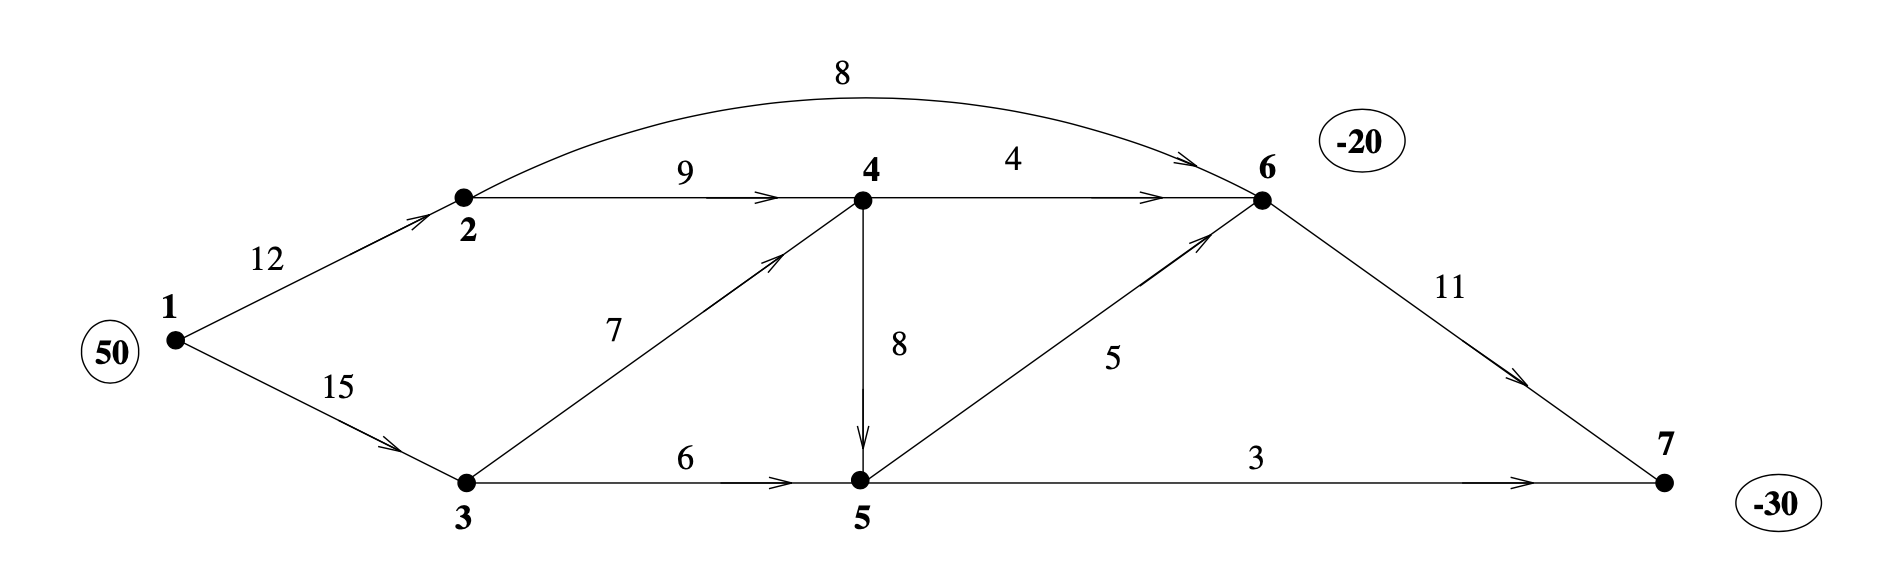
\includegraphics[width=.90\textwidth]{SampleNetwork.png}
  \end{center}
\end{figure}



If a vertex has positive flow we call it a source, and if vertex has negative flow we call it a sink. 
We define Supply, $S$ as 
\begin{equation*}
  S = \sum_{\{i :b_i > 0\}}b_i,
\end{equation*}
and Demand, $D$ as
\begin{equation*}
  D = \sum_{\{i: b_i < 0\}}b_i.
\end{equation*}
We call a network balanced if $S + D = 0$, and an unbalanced network can be made balanced by adding an artificial vertex with flow $S - D$ by a directed edge with 
zero cost.\\


The goal of the minimum cost network flow problem is to satisfy the supply and demand of each vertex while minimizing the cost. Naturally the objective function will look 
like this, 
\begin{equation*}
    \mathop{\text{minimize: }}_{x}  z = c^Tx
\end{equation*}
where $x_{i,j} \in x$ represents the amount of flow through arc $(i, j)$, and we denote $c_{i, j}$ as the cost assigned to arc $(i, j)$. It's important to note that at the moment we are thinking of $x$ and $c$ as vectors, so this indexing is just for identifying 
the corresponding arc, not some location on a matrix. A feasible solution to this problem is an $x$ which satisfies the supply and demand of each vertex. 
With that context at each vertex $i$ our $x$ must satisfy, 
\begin{equation*}
  \sum_{j}x_{i, j} - \sum_{k}x_{k, i} = b_i.
\end{equation*} 
One can think of the first sum being flow out of vertex $i$ and the second sum being flow into vertex $i$. As an example consider vertex $1$ and $2$ in Figure 1, 
we get the following constraints
\begin{equation*}
  x_{1, 2} + x_{1,3} = 50,
\end{equation*}
\begin{equation*}
  x_{2, 4} + x_{2, 6} - x_{1, 2} = 0.
\end{equation*}
This is done for each vertex $i$, generating our constraint matrix $A$ which will be size (\# of vertices)$ \times $(\# of edges). Usually there will be some added constraints $L$ and $U$ on the amount of flow that can go through each edge (Capacity!!), so most problems will be of the form, 
\begin{align*}
    \mathop{\text{minimize: }}_{x}  z &= c^Tx\\
  \text{subject to: }Ax &= b\\
  L \leq&x\leq U
\end{align*}
At this moment I urge you to have an internal dialogue about the well-posedness of such a problem, specifically for a given $U$ which is small, and an assignment of flows $b$ which is very large. (This situation has a name and we typically call a $LP$ problem \emph{infeasible} when this happens)


\subsection{Maximum Flow}
Suppose you have a directed graph with $m$ vertices but in this case, we only consider two special vertices, $1$ and $m$ where $1$ is 
the source and $m$ is the sink. The weights assigned to each arc represent the maximum capacity of flow that can move between vertices. \\


The goal of a maximum flow network problem is to maximize the amount of flow through the source and the sink without overwhelming the capacity of the network. So a solution to the maximum flow network problem determines the maximal amount of flow that can be moved from source to sink, as well as the routing of that flow across the network. 

To formulate the problem as a linear program, as before let $x_{i, j} \in x$ represent the amount of flow through arc $(i, j)$, let $u_{i, j}$ represent the capacity of arc $(i, j)$. Let $f$ be the amount of flow in the network. Then our problem can be written in the following form, 
\begin{align*}
    \mathop{\text{maximize: }}_{x, f} &z = f\\
    \text{subject to: } &\sum_{j}x_{1, j} - \sum_{k}x_{k, 1} = f,\\
    &\sum_{j}x_{i, j} - \sum_{k}x_{k, i} = 0, \quad i = 2, \dots, m - 1\\
    &\sum_{j}x_{m, j} - \sum_{k}x_{k, m} = -f,\\
    &0 \leq x_{i, j} \leq u_{i, j}.
\end{align*}
Naturally since we wish to find the maximum flow $f$, between vertices $1$ and $m$ through the network, vertex $1$ will have a surplus of flow $f$ and 
$m$ will have a demand of flow $f$. Since all the flow is moving from $1$ to $m$ all vertices in between must be balanced, hence the 0 on the right hand side of the middle equality constraints. Finally the inequality constraints come from our desire to not overwhelm the capacity of the network. 

We can convert the maximum flow problem into a minimum cost network flow problem. Suppose we add an an artificial arc $(m, 1)$ with unlimited 
capacity $u_{1, m}$. Then the problem can reformulated by, 
\begin{align*}
    \mathop{\text{minimize: }}_{x} &z = -x_{m, 1}\\
    \text{subject to: } &\sum_{j}x_{i, j} - \sum_{k}x_{k, i} = 0, \quad i = 1, \dots, m\\
    &0 \leq x_{i, j} \leq u_{i, j}
\end{align*}
To see this let $x_{m,1} = f$ and by substitution the constraints are equivalent. Since minimum cost network flow is a minimization problem we multiply the cost function by $-1$, hence $z = -x_{m, 1}$. To see this in the previously stated matrix vector form of the minimum cost network flow problem, let $b = 0$, let $c$ be a one hot vector with $c_{m,1} = -1$, let $L = 0$ and, let $U = u$ a vector of arc capacities. Note that the cost $c_{i, j} = 0$ for all edges in our graph other than our strategically placed artificial arc, and recall that throughout our discussions of this problem in class, there was never any mention of costs across edges. (I suspect they were there all along...) %\smiley{})

\subsection{Minimum Cut}
Since we've described the maximum flow problem as an $LP$ problem, we can easily convert it to standard form and construct its dual $LP$ problem. From our discussions in class, strong duality states that such a dual should compute the minimum cut on this network, let's verify that for ourselves. Since I've suppressed the details of how to convert a $LP$ problem to standard form, I'll simply present you with the dual of the original problem and argue it produces the minimum cut,
\begin{align*}
    \mathop{\text{minimize: }}_{y, v}  &w = \sum u_{i, j} v_{i, j}\\
    \text{subject to: } y_m - y_1 &= 1\\
    y_i - y_j &+ v_{i, j} \geq 0, \quad \text{for all arcs $(i, j)$}\\
    v_{i, j} &\geq 0
\end{align*}
First let's define $N_1$ and $N_0$ to be the independent sets of vertices. We would like our dual variable $y_i$ to encode when a vertex is in either $y_i \in N_1$ or $y_i \in N_0$. In order to satisfy the first constraint it is clear that $y_m = 1$ and $y_1 = 0$ as desired since our source and sink must be separated. We interpret the second dual variable $v_{i, j}$ as an indicator for if an arc is in the cut set, so $v_{i, j} = 1$ if $i \in N_1$ and $j \in N_0$, and $v_{i, j} = 0$ otherwise. We are pleased to find that the objective is what we expect, minimizing a sum of capacities over arcs in the cut set. Now finally if $y_i \in N_0$ and $y_j \in N_1$ we force $y_i - y_j = -1$ and in order to stay feasible $v_{i, j} = 1$, hence we get the desired quality for our indicator $v_{i, j}$. A similar argument show that arcs between vertices in the same set, can be added to the cut set as well. 


\subsection{Shortest Path}
The shortest path problem can be represented very simply as a minimum cost network flow problem. First you construct the directed graph in the obvious way to model the physical network you are trying to traverse. The starting source vertex, is ascribed a flow of 1, and the ending sink vertex with a flow of -1, defining the $c_{i, j}$ as the distance between vertices $i$ and $j$. 

As an aside it should be noted that there are several especially efficient algorithms for solving the shortest path problem (A* and Dijkstra's come to mind), and this formulation via a minimum cost network flow problem is by no means any better (the method in the appendix is a polynomial time algorithm). However it is more general, in the sense that the more popular algorithms require that the cost $c_{i,j} \geq 0$ and our formulation allows us the case where $c_{i, j} < 0$ as well. (in fact it was only recently found that such a negative weight efficient near-linear time shortest path algorithm exists.)  


\subsection{Assignment} 
Let's recall the premise of the stable matching problem, where a collection of medical students are applying to medical residencies and say instead of creating a list of preferences the students decide to ascribe a happiness score $c_{i, j}$ for which the $i^{th}$ student would attain should they be accepted to the $j^{th}$ program. You can think of this as a sort of weighted preference list. The goal of the assignment problem is to assign each student to a program, and maximize the total amount of 'happiness'. 

Again the graph is constructed in the usual way, as a complete bipartite graph with one part representing students and another representing medical residencies (it is necessary to have equal parts). Every student source vertex is ascribed a flow of 1, and every school sink vertex with a flow of -1. We assign the costs as expected using the happiness score $c_{i, j}$, however this time we want to maximize the objective function. 



\section{Applications in Image Segmentation}

Extending our discussion of Flow Problems, I'd like to discuss a particularly interesting application of the Max-Flow/Min-Cut problem in the field of computer vision. Image segmentation is the process by which the subject and background of an image are identified. To apply our knowledgeu about flow problems we would hope to define a graph where each vertex represents a pixel or some portion of the image and capacities, source vertices, and sink vertices such that the Min-Cut separates our subject from the background. 

This idea is called 'Lazy Snapping' and it works by first presenting a user with an image, the user then selects a small portion of the subject in the image to be source pixels, and another portion of the background to be sink pixels. Then the goal is to, find the assignment $X$, of pixels into two classes where $X(x_i) = 1$ (subject) or $X(x_i) = 0$(background) which minimizes the following energy function, 
\begin{equation*}
    E(X) = \sum_{i \in V} E_1(x_i) + \lambda \sum_{(i, j) \in E} E_2(x_i, x_j). 
\end{equation*}
There is a substantial amount of details which I will suppress, but essentially $E_1$ is defined in such a way that $\sum_{i \in V} E_1(x_i)$ is small if pixels of the same class are the same color. Also $E_2$ constructed such that it only takes on positive values for which $x_i$ and $x_j$ are in different classes otherwise it is zero, and it is larger when the two colors are similar and smaller when they are dissimilar. Having described the energy function in this way there should be a feeling that minimizing $E$ must separate a subject from its background. Actually producing the capacities for such a graph and proving that the Min-Cut algorithm minimizes this energy function will be left to the following references. Expect details and a demo during my presentation.
\newpage









\appendix
\section{Network Simplex}
\subsection{Feasibility}
The crux of the network simplex method lies in two key ideas and we will explore them in the context of a 
minimum cost network flow problem with only positivity constraints. Let $G = (V, E)$ be a network on $m$ vertices and recall the minimum cost network flow problem, 
\begin{align*}
    \mathop{\text{minimize: }}_{x}  z &= c^Tx\\
  \text{subject to: }Ax &= b\\
  x \geq& 0
\end{align*}
By our definition of $x_{i, j} \in x$ as the flow between arc $(i, j)$ we know that the columns of our constraint matrix $A$ represent 
the arcs in our network. Since we constructed each row of our matrix $A$ is an equation which models the flow across a single vertex, we know that each row represents a vertex. So in the column view, a column representing arc $(i, j)$ will have a $1$ in the row representing vertex $i$ and a $-1$ in the row representing 
vertex $j$. In the row view, a row representing vertex $i$ will have a $1$ in every column representing arc $(i, k)$, and a $-1$ in every row representing arc $(k, i)$ where 
$k \in V$ hence the constraint matrix is a directed incidence matrix. The first big idea comes as the following theorem.
\begin{theorem} Let $B$ be a submatrix of the constraint matrix $A$ whose columns represent the edges of a spanning tree.
    Then $B$ is a full column rank matrix with dimension $m \times (m - 1)$, and it can be rearranged so that the diagonal entries are $\pm 1$. 
\end{theorem}

There is a sense that this result feels intuitive, clearly a spanning tree on a connected graph with $m$ vertices must have $m - 1$ arcs. Showing that 
$B$ can be rearranged follows by a proof by induction (you can find it on p.285 of Griva). 

% Maybe write it out

Recall that a basic solution $x$ to a general LP problem has non-zero entries, whose corresponding columns in the constraint matrix $A$ are linearly independent
and $x$ satisfies the equality constraints. We define a \emph{spanning tree solution} $x$, as a solution to the system $Ax = b$ where the non-zero entries of $x$
correspond to columns of $A$ which represent a spanning tree. A \emph{feasible spanning tree solution} is simply a spanning tree solution which also satisfies the 
positivity constraints, $x \geq 0$. The next big idea uses the previous theorem and definitions about spanning trees and connects them to LP, 
  
\begin{theorem} A flow $x$ is a basic feasible solution for the network flow constraints $Ax = b$ and $ x \geq 0$ if and only if it is a feasible spanning tree solution.  
\end{theorem}
The backwards direction follows directly from the previous Theorem 1 and the definition of feasible spanning tree solution. The forwards direction proceeds by contradiction supposing 
$x$ is a basic feasible solution and not a feasible spanning tree solution. If 
$x$ is not a spanning tree then it must have a cycle. Choose a vertex $i$ in the cycle, it must have arcs $(i, j)$ and $(k, i)$ for some $k$ and $j$ in the cycle.
The flow across an arc $(i, j)$ in the cycle may be increased by some $\epsilon \geq 0$, and in order to stay feasible we must decrease the flow across the arc $(k, i)$. 
So we have a new flow $x_\epsilon$, we can construct another flow $x_{-\epsilon}$ by subtracting $\epsilon$ from the flow across $(i, j)$ and adding $\epsilon$ to $(k, i)$.
%% Add image. 
Finally note that, 
\begin{equation*}
    x = \frac{1}{2}x_{\epsilon} + \frac{1}{2}x_{-\epsilon}.
\end{equation*}
Therefore $x$ is not an extreme point in the feasible set and by the Fundamental Theorem of Linear Programming $x$ is not a basic feasible solution. 

\subsection{Network Simplex} 
The network simplex method proceeds in a similar fashion, to the general simplex method with a few improvements on how we 
compute each step. First note that we must initialize the algorithm, just like the regular simplex method with basic feasible solution. One could 
conceivably implement the first step problem to find a BFS. Like in the regular simplex method we'll need to form our Basis and Null matrices $B$ and $N$
respectively. As we have shown in the previous section our $B$ matrix will be full column rank with dimension $m \times (m - 1)$ and the $N$ matrix 
will have columns which represent all the arcs that didn't show up in our feasible spanning tree. Recall that the first step in the simplex method is to compute
simplex multipliers $y$ by solving the system, 
\begin{equation*}
    B^Ty = c.
\end{equation*}
Here is where we can take advantage of Theorem 1 to make solving this system faster. Note that $B^T$ is a full row 
rank $(m - 1) \times m$ matrix, so we are guaranteed when solving $B^Ty = c$ to have a free variable. Since $B^T$ is 
a matrix whose rows now represent edges, solving this system by back substitution produces the following expression, 
\begin{equation*}
    y_i - y_j = c_{i, j}
\end{equation*} 
where $y_i$ and $y_j$ are the simplex multipliers associated with vertices $i$ and $j$ and $c_{i, j}$ is the cost associated to 
arc $(i, j)$. This means that we can compute the simplex multipliers by selecting a vertex $i$ to correspond to our free simplex multiplier, so we will let $y_i = 0$ 
and we compute the rest $y_j$ by traversing the feasible spanning tree computing $y_j = y_i - c_{i,j}$ along the way.  


Computing the reduced costs is no different from the regular simplex method, we use $\hat{c}_{i, j} = c_{i, j} - N^Ty$. Again choosing which arc becomes the new entering arc is no different, 
simply find the minimum $\hat{c}_{i, j}$ and consider the corresponding arc $x_{i, j}$ in the columns of $N$. Then we check our optimality conditions just as before, are $\hat{c}_{i, j} \geq 0$. 


To choose our leaving arc, we will be taking advantage of Theorem 2 and a small result about spanning trees. Taking our entering arc $x_{i, j}$ and adding it into our spanning tree graph, it is 
guaranteed that this will produce a single undirected cycle that includes the arc $x_{i, j}$. By Theorem 2 adding this arc $x_ {i, j}$ into our solution makes us no longer basic. 
In order to stay feasible and basic, we must remove an arc from the cycle to get back to a spanning tree, and increase the flow through $x_{i, j}$ and appropriate amount to satisfy our equality constraints. Here's the trick, 
locate the edges in the cycle which point in the opposite direction as $x_{i, j}$, we'll call them negative edges. Let $m$ be the minimum flow through those negative edges. Set $x_{i, j} = m$ and 
subtract $m$ from all negative $x_{l, k}$ in the cycle. This operation maintains basic feasibility since the minimum flow $x_{l, k}$ arc gets removed from our solution becoming our exiting variable and our 
entering variable in increased enough to satisfy the equality constraints. Also note that if there is no minimum flow $x_{l, k}$, and $x_{i, j}$ can be increased arbitrarily than
the problem is unbounded, just like in the regular simplex method. 

The steps are then repeated with the new feasible spanning tree solution until we achieve the optimality conditions. 


\section{Implementation} Consider the example defined in Figure 2, of a positively constrained minimum cost network flow problem.
\begin{figure}
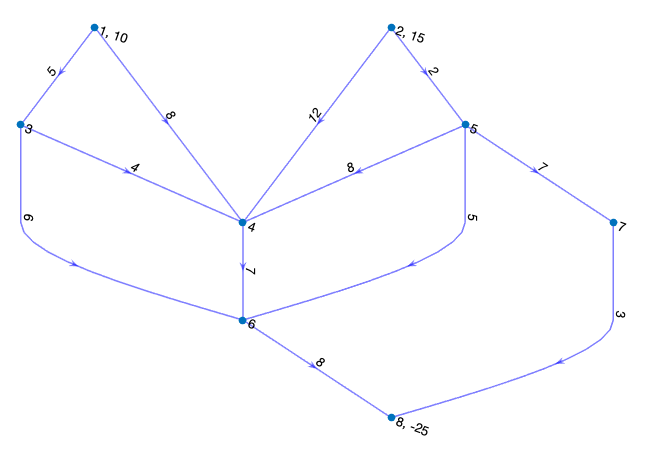
\includegraphics[width=.80\textwidth]{untitled.png}  % put image "foo.png" in current directory
\caption{Our given network which defines $A$ and $b$, by network structure and flow. }
\end{figure}

\begin{figure}
    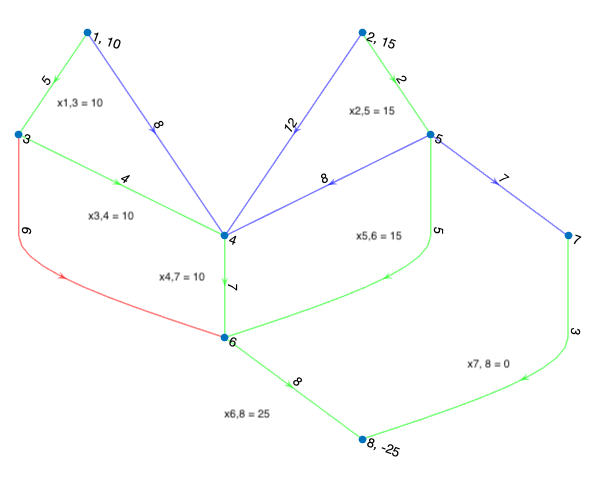
\includegraphics[width=.80\textwidth]{step1.png}  % put image "foo.png" in current directory
    \caption{Initial feasible spanning tree shown in green. Red is the entering arc for this first iteration.}
    \end{figure}
    Our initial feasible spanning tree solution outlined in green in Figure 3. Again the equations for computing the simplex multipliers allows us to simply set 
    the multiplier associated with vertex 1 to zero, so we get $y_1 = 0$. To solve the next multiplier we traverse the green spanning tree to vertex 3 and in doing so we solve 
    for $y_3$ with $y_3 = y_2 - c_{1,3} = 0-5 = -5$. Solving the next multiplier we get $y_4 = y_3 - c_{3, 4} = -5 - 4 = -9$ and so on. 

    Once we have the simplex multipliers together we can solve for the reduced costs of the nonbasic arcs. Doing so we can check our optimality conditions, and in this 
    case there exists negative reduced costs, so we continue. You'll find that the reduced cost for $x_{3, 6}$ (marked in red in Figure 3) is the lowest among the negative reduced costs and therefore becomes our 
    entering arc. 

    To solve for our exiting arc consider the cycle formed by vertices $\{3, 4, 6\}$. Note that $x_{3, 6}$ is pointing in the counter clockwise direction, and therefore we designate 
    arcs $x_{3, 4}$ and $x_{4, 6}$ as negative. Note that the minimum flow across the negative arcs is equal so when we subtract that flow from $x_{3, 4}$ and $x_{4, 6}$ and 
    add it to $x_{3, 6}$ both $x_{3, 4}$ and $x_{4, 6}$ will be zero and we will get to choose which of the two arcs becomes our exiting arc. 
    Choosing $x_{3, 4}$ to be the exiting arc and setting $x_{3, 6} = 10$ we arrive at the next feasible spanning tree solution. Figure 4 shows the final iteration of this problem, the working out is 
    left as an exercise to the reader.   
    \begin{figure}
        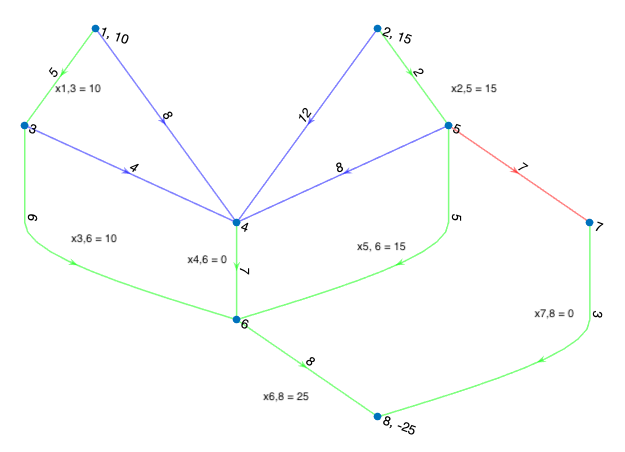
\includegraphics[width=.80\textwidth]{step2.png}  % put image "foo.png" in current directory
        \caption{In green is the resultant spanning tree from the first iteration. In red is the next entering arc for the second iteration.}
        \end{figure}

    You'll find code and an example, for running this method on positively constrained minimum cost flow network problems on my github page. 


\begin{thebibliography}{2}  % "2" because there are two references use  \cite{einstein}
\bibitem{grivanashsofer}
I.~Griva, S.~Nash, \& A.~Sofer (2009).
\textit{Linear and Nonlinear Optimization},
2nd ed., SIAM Press.

\bibitem{Boykov}
Boykov, Y.Y., and M.-P. Jolly. “Interactive Graph Cuts for Optimal Boundary \& Region Segmentation of Objects in N-D Images.” In Proceedings Eighth IEEE International Conference on Computer Vision. ICCV 2001, 1:105-12. Vancouver, BC, Canada: IEEE Comput. Soc, 2001. https://doi.org/10.1109/ICCV.2001.937505.

\bibitem{yin}
Li, Yin \& Sun, Jian \& Tang, Chi-Keung \& Shum, Heung-Yeung. (2004). Lazy snapping. ACM Trans. Graph.. 23. 303-308. 10.1145/1015706.1015719. 

\bibitem{Bernstien}
Bernstein, Aaron, Danupon Nanongkai, and Christian Wulff-Nilsen. “Negative-Weight Single-Source Shortest Paths in Near-Linear Time.” arXiv, October 30, 2022. https://doi.org/10.48550/arXiv.2203.03456.

\end{thebibliography}



\end{document}
